\section{Our Current Data Disguising Framework}

We propose \emph{data disguising}, a systematic approach to privacy transformations that separates
them from application code. We believe data disguising systems can help support flexible privacy
transformations and reversibility.
%
Data disguising represent privacy transformations as structured \emph{disguises} that are specified
by the developer to capture application-specific policies.
%
Applications invoke an external data disguising tool's API to trigger disguise application; the tool
interprets and applies the necessary physical changes to the application database.
%
Data disguising offers mechanisms to handle multiple disguise interactions and reversible disguises
in the form of automatically-generated \emph{revealing functions} stored in \emph{vaults}.

%
%In the following, we sketch one design for a data disguising framework.
%
%Some of the specific design decisions in this framework have alternatives that are worth
%investigating, and open research questions remain; we discuss these in \S\ref{s:disc}.

\subsection{Disguises: Structured Privacy Transformations}
\label{sec:disguises}

\begin{figure}[t]
    \centering
    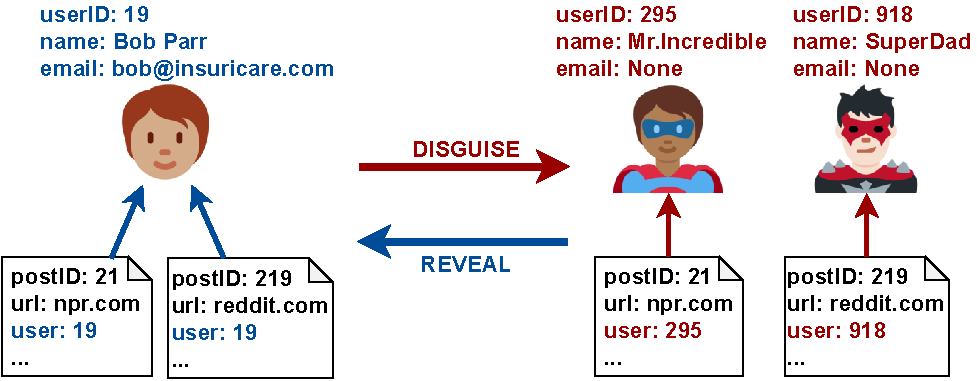
\includegraphics[width=0.47\textwidth]{img/disguises_new}

    \caption{A user deletion disguise decorrelates user Bob from his posts while maintaining
    referential integrity by replacing his profile with anonymous placeholders.}
    \label{fig:example}
\end{figure}

\begin{figure}[t!]
    \centering
    \footnotesize
\begin{lstlisting}[language=Rust]
disguise_name: "AccountDeletion",
user_to_disguise: 19,
tables {
   User: {
      generate_guise_info: [
         ("name", Random),
         ("email", Default(None)),
         ..
      ],
      transformations: [Remove(pred: "userID" = UID)]
   },
   Post: {
      transformations: [Decorrelate(
         pred: "userID" = 19,
         foreign_key: ("user", User)
      )],
   }
}
\end{lstlisting}
    \caption{Specification of an account deletion disguise.}
    \label{fig:spec}
\end{figure}

The broad range and application-specific nature of privacy transformations poses a real
implementation challenge. We believe that data disguising makes
privacy transformations more manageable by separating them from application code,
and organizing them as structured, automatically-applicable \emph{data disguises}.

Data disguises are built on three fundamental operations---data removal, object content
modification, and decorrelation by modifying references between objects---that can capture and
structure many desirable privacy transformations across applications.
%
The application developer writes a disguise specification for each of the application's privacy
transformations; this specification consists of predicated operations on each table, and describes
the necessary operation(s) to perform on objects satisfying the predicate (Figure~\ref{fig:spec}).
A data disguising tool takes the disguise specification and turns it into storage operations that
achieve the desired application data state.

Figure~\ref{fig:example} illustrates how the tool performs the example user
account deletion disguise for Bob, when given the disguise spec in Figure~\ref{fig:spec}.
%
When his account is active, Bob's profile is associated with his true identity and all his
contributions to the site.
%
When Bob deletes his account, his profile and contributions move to different, privacy-preserving
placeholders: 
%his name has been anonymized, his email address has been redacted, and 
his contributions have been decorrelated and attributed to individual, unidentified user guises, 
making it seem as if a different user provided each of Bob's contributions.
%
This allows these contributions to be retained, but prevents an observer from correlating these
contributions back to Bob's identity, and 
importantly preserves refential integrity in the database, a precondition to application
correctness.

\lyt{Should add stuff about FK traversal? (It's not a huge part of the current
design/implementation)}

%
%Disguises transform a guise by modifying it at per-attribute (\ie per-column) granularity, or
%splitting it into multiple guises in order to decorrelating from objects that reference it (via \eg foreign-key relationships).
%
%Guises can also be removed entirely.
%
%At any given moment, an application's data comprises a mix of identity-revealing guises
%and privacy-preserving ones. Disguises modify, split, and/or combine individual guises when triggered.

%-------------------------------------------------------------------------------
\subsection{Handling Disguise Interactions}
%\label{sec:composition}
%-------------------------------------------------------------------------------

Applications have specific privacy goals that should be achieved by a disguise,
but this is complicated by interactions between different disguises and reversible disguises.
%
Because disguises inherently destroy data, applying one disguise may change the outcome of future
disguises applied on top of it.

For example, consider two desirable disguises in HotCRP: \gdpr and \ca.
%
\gdpr removing the user's data to comply with the GDPR's ``right to be forgotten''; \ca provides
user privacy by anonymizing all conference data.
%
These disguises touch the same data: applying \ca destroys information that \gdpr would remove
or transform if applied to an unmodified database.
%

%
In some cases, the disguises compose naturally---\eg information that an earlier disguise removed
needs no decorrelation---but in others, the tool may need to reveal the original data to meet the
application's privacy goals. Even then, the necessary actions depend on the specific application:
some applications may require that previously anonymized data still be deleted, while other
applications may not.
%

Data disguising provides the infrastructure and mechanisms to reveal data to support 
disguise composition and disguise reversibility; however, appropriate use of these to
achieve application privacy goals remains an open challenge, which we discuss in \S\ref{s:disc}.
%To handle inter-disguise dependencies, a disguising tool relies on (1) the structured nature of
%disguises to
%statically determine whether disguises share dependencies, and (2) the key abstraction of \emph{user
%vaults}, namely per-user logs of disguise updates to that user's data.  User vaults solve the issue
%that disguises inherently destroy data necessary to correctly achieve the end-state of future
%disguises by providing a secure way to store the data. A disguising tool queries the user vault to
%temporarily restore destroyed data (\eg decorrelated foreign key relationships) in order to apply
%the disguise correctly.

%As shown in Figure~\ref{fig:tool}, a disguising tool sits next to the application, and queries the
%user vaults and the application database. The application performs disguises by invoking a
%disguising tool.

%-------------------------------------------------------------------------------
\paragraph{Vaults.}
%-------------------------------------------------------------------------------

Vaults provide the necessary infrastructure to reveal previously-disguised data when
necessary
%, either for temporary data for disguise composition, or for reversing a disguise entirely.
%
They store \emph{revealing functions} for disguises, which when applied, reveal the underlying
data transformed by an already-applied disguise (possibly temporarily). These functions are
automatically produced by the disguising tool when a disguise is applied.
%

%
Vaults can be flexibly configured and deployed. It remains important, however, that any
configuration of vaults should not violate the guarantee that disguises indeed destroy data,
from the viewpoint of the application and any users.
We imagine several exciting directions to explore for designing vaults that are both
performant and secure.
%

%
Some possible configurations include a disguising tool storing per-user vaults encrypted with a per-user key; this key
may be secret-shared using a (2, 3) threshold scheme~\cite{secretsharing} between the user, the
tool, and a trusted third party (\eg Amazon S3), so that the user can authorize a disguising tool and the
third party to restore the key if the user forgets their share.
%
The vault entries could be configured to expire after a certain time; the corresponding disguises
then become irreversible.
%
Or perhaps the vault entries are stored entirely by some third party or locally by the user, whose
server runs a corresponding interface to allow disguise tools to read and write the vault.

The choice of vault deployment has serious consequences for the practicality of disguise reversal.
For example, if \gdpr is to be reversable, reveal functions must necessarily be stored in per-user
vaults external to the application in order to be GDPR-compliant.  While it is reasonable to imagine
accessing a single user's vault to reverse \gdpr in this deployment, complete reversal of \ca would
need to retrieve reveal functions from every user's vault, an infeasible task.
%
An alternative might be a multi-tier security design: the first tier stores reveal functions of
non-GDPR disguises in a global vault acccessible to the disguising tool and application, while the
second tier stores reveal functions from user-invoked disguises in external, per-user encrypted
vaults.

%-------------------------------------------------------------------------------
\paragraph{Revealing Data.}
%-------------------------------------------------------------------------------
\lyt{I feel like this sticks out, but it is a reasonable part of our solution to handling disguise
reversal.}
When disguises are explicitly reversed, this permanently reveals data to the application database.
However, in the interval between disguising and revealing the data, other disguises may have been applied that
should have affected the newly reintroduced data. To ensure that any revealed data is properly disguised,
the disguising tool keeps a persistent log of all disguises performed by the application, and
applies to this data any disguises performed in this interval.

For example, reversal of \gdpr should not reintroduce ownership of reviews to identities if \ca has
occurred since \gdpr was applied. The data disguising tool would applying the relevant \ca
anonymization operations to any revealed data from \gdpr's reversal before making it visible to the application.

%\ms{OLD TEXT FOLLOWS}

\iffalse
%For example, Figure~\ref{fig:example} would include a specification that all email
%addresses be obfuscated in an anonymous manner for the user with name ``Bob Parr''.
%
%Transformations can either remove objects, or change objects into one or more guises.
%To create a guise from an object, developers specify how to transform attributes of the
%object (\eg table column values) into guise attributes (\eg changing email addresses).

%
%When writing a disguise, developers can reason about its
%specification in isolation; interactions between different disguises are handled by a disguising
%tool (\S\ref{sec:composition}).
%
%We assume that:
%\begin{enumerate}[nosep]
%  \item developers use their domain knowledge to write correct and complete disguises;
%      \lyt{should make clear that correct/complete is just operational? \eg doesn't mess up the DB}
%  \item application code handles the different guises appropriately (\eg in
%    displaying them); and
%  \item different guises of the same object have the same structure (\eg they can be
%    rows in the same table).
%\end{enumerate}
%
Developers choose how to create other guise attributes, selecting from among the following:
%
\paragraph{(1) Copy object content.}
%
Guises of the same object all share the object's attribute values.
%
If the attribute is a reference attribute (\eg a foreign key column), all guises will refer to the same object.
%
%
Copying allows developers to retain the object's content, without worrying about how to
synthesize attribute values for guises.
%
%However, this should only be chosen if guise attribute
%values cannot be generated, or if this attribute says little about the true identity of the
%entity.
For example, in Figure~\ref{fig:guises} the \texttt{darkmode} attribute is copied in
all guises.
%; the \texttt{darkmode} attribute reveals very little about the underlying user's
%identity.

\paragraph{(2) Generate new content.}
%
To create new attributes, developers specify whether the guise's value should be random,
a default value, or generated from the object's attribute value via a custom function (\eg hashing
the value).
%
Figure~\ref{fig:guises} illustrates an example of random (\texttt{name}) and default
(\texttt{active}) generated value attributes.
%
%
Creating new guise reference attributes (\eg new foreign key relationships) requires
creating a new guise for the referenced object in order to maintain referential
integrity;
the data disguise rewrites the reference to point to the new guise.
%
In Figure~\ref{fig:guises}, creating two user guises requires creating two
tag guises, and the tag guises' identifiers become the user guises' foreign keys.
%

\paragraph{(3) Copy object content, but only once.}
%
One guise copies the attribute value from the object, but all other guises generate new
values (as described above).
%
\texttt{notifs} in Figure~\ref{fig:guises} illustrates how the attribute is copied once.
%
This enables the application to retain the original object semantics (\eg a count of how many
users want notifications) without creating duplicates.
%



\begin{figure*}[t!]
    \centering
    \footnotesize
\begin{tabular}{@{}c|c|c|c@{}}
\textbf{User Transformation Spec} & \textbf{User Object} & \textbf{Guise 1} &
    \textbf{Guise 2} \\
\begin{lstlisting}[language=Rust]
"id":       IDAttribute,
"name":     Gen(Random),
"active":   Gen(Default(false)),
"darkmode": CopyAll,
"notifs":   CopyOnce+Gen(Default(false)),
"tag_id":   GenForeignKey,
\end{lstlisting}
    &
\begin{lstlisting}[language=Rust]
"id":       19,
"name":     BobParr,
"active":   true,
"darkmode": false,
"notifs":   true,
"tag_id":   11
\end{lstlisting}
&
\begin{lstlisting}[language=Rust]
"id":       295,
"name":     MrIncredible,
"active":   false,
"darkmode": false,
"notifs":   true,
"tag_id":   81483
\end{lstlisting}
&
\begin{lstlisting}[language=Rust]
"id":       918,
"name":     SuperDad,
"active":   false,
"darkmode": false,
"notifs":   false,
"tag_id":   15592
\end{lstlisting}
\end{tabular}
    \caption{Creating two guises of an example user (of a synthetic application schema).}
    \label{fig:guises}
\end{figure*}


%-------------------------------------------------------------------------------
\paragraph{Applying Disguises.}
%-------------------------------------------------------------------------------
A disguising tool applies disguises in a five-phase procedure:
\begin{enumerate}[nosep]
    \item \emph{Prepare}: execute the appropriate reveal functions of co-dependent,
        reversible disguises from the user vaults, if applicable (\S\ref{sec:composition})
        %reconcile any data dependencies between this disguise and prior disguises.
        %A disguising tool detects read-after-write dependencies between the new disguise's
        %predicates and prior disguises' updates, and, using entries in the vault, undoes any writes
        %that may affect the new disguise's predicates. As an optimization, vault entries recording
        %object removals need not be reversed.
        \item \emph{Read}: get all objects that satisfy (per-type) developer-specified predicates.
        \item \emph{Update}: modify, decorrelate, or remove objects read in step (2) according to the
        developer's specification.
    \item \emph{Record}: if the disguise is reversible, store per-user reveal functions for the
        disguise in the appropriate per-user vaults.
        A disguising tool must be able to determine which user vault should record each modification. This can be
        developer-specified, or rely on a set of heuristics (\eg assigning ownership by traversing,
        starting from each user, the application's object graph expressed in an object-relational
        model (ORM)~\cite{orm}, or implicitly via foreign keys).
        \item \emph{Finalize}: After applying the new disguise updates, the disguising tool
            redisguises any temporarily revealed data from earlier disguises.
\end{enumerate}

%Composed disguises should achieve an end-state that combines, in some way, the end-states achieved by each disguise when applied to the original application database in isolation.
%Correct composition of multiple disguises achieves an end-state equivalent to combining the
%end-states achieved by each disguise when applied to the original application database in isolation.
%
%If a prior disguise is reversible, then a disguising tool can use user vaults to ensure that this
%prior disguise does not affect \emph{which} objects are updated
%a future disguises.
%%In this case, a disguising tool allows developers to reason about multiple conflicting updates to
%the same object:
%regardless of when the disguises occurred, if one disguise removes an object that the other disguise
%modified, then the removal takes precedence.
%%
%
%However, if they both modify the same object attribute, a disguising tool establishes no precedence
%between the modifications and applies them in chronological order.  Alternatively, we can imagine
%that the developer could specify a partial ordering between modifications, or our framework could
%restrict the set of possible modifications and establish a precedence order within this set.
%
%If the prior disguise is not reversible, however, then the disguising tool could prevent future
%conflicting disguise application, or perhaps a-priori prevent the application of such non-reversible
%disguises that conflict with legally required disguises such as GDPR deletion \lyt{not sure what to
%put here? May also want to include something about developer assertions}
%%: a disguise will update all objects that it would have updated if performed on
%the original, undisguised state of application data.


\fi
